\documentclass{beamer}
%%% Обязательные пакеты
%% Beamer
\usepackage{beamerthemesplit}
\usetheme{spbu}
\beamertemplatenavigationsymbolsempty
\usepackage{appendixnumberbeamer}
%% Локализация
\usepackage[T2A]{fontenc}   % кириллические шрифты Type 1
\usepackage[utf8]{inputenc} % источник: файл в UTF-8
\usepackage[russian,english]{babel}
\usepackage[autostyle]{csquotes} % Правильные кавычки в зависимости от языка
%% Графика
\usepackage{wrapfig} % Позволяет вставлять графику, обтекаемую текстом
\usepackage{pdfpages} % Позволяет вставлять многостраничные pdf документы в текст
%% Математика
\usepackage{amsmath, amsfonts, amssymb, amsthm, mathtools} % "Адекватная" работа с математикой в LaTeX
% Математические окружения с русским названием
\newtheorem{rutheorem}{Теорема}
\newtheorem{ruproof}{Доказательство}
\newtheorem{rudefinition}{Определение}
\newtheorem{rulemma}{Лемма}
%%% Дополнительные пакеты. Используются в презентации, но могут быть отключены при необходимости
\usepackage{multirow} % Ячейка занимающая несколько строк в таблице
%% Пакеты для оформления алгоритмов на псевдокоде
\usepackage[noend]{algpseudocode}
\usepackage{algorithm}
\usepackage{algorithmicx}
\usepackage{fancyvrb}
%% Пакет для анимированных иллюстраций
\usepackage{animate}
\usepackage{cmap}
% То, что в квадратных скобках, отображается внизу по центру каждого слайда. 
\title[Непрерывное обучение с KAN]{Исследование эффективности непрерывного обучения с
использованием сетей Колмогорова-Арнольда в задаче распознавания образов}
% То, что в квадратных скобках, отображается в левом нижнем углу. 
\institute[СПбГУ]{}
% То, что в квадратных скобках, отображается в левом нижнем углу.
\author[Третьяков Даниил]{Третьяков Даниил Александрович, группа 21.Б07-пу}
 \begin{document}
{
\setbeamertemplate{footline}{}
% Лого университета или организации, отображается в шапке титульного листа
\begin{frame}
  
\includegraphics[width=1.4cm]{figures/spbu_logo.png}
\vspace{-35pt}
\hspace{-10pt}
\begin{center}
   \begin{tabular}{c}
        \scriptsize{Санкт-Петербургский государственный университет} \\
        \scriptsize{Кафедра системного программирования}
    \end{tabular}
\titlepage
\end{center}
\btVFill
\vspace{-269pt} % Иначе название работы вытесняет дату за границы слайда
{\scriptsize
  \textbf{Научный руководитель:} профессор кафедры компьютерного моделирования и
    многопроцессорных систем, д.т.н. Дегтярев Александр Борисович\\

  \textbf{Рецензент:} доцент кафедры компьютерного моделирования и
    многопроцессорных систем, к.ф.-м.н. Корхов Владимир Владиславович\\
}
\begin{center}
  \vspace{5pt}
  \scriptsize{{Санкт-Петербург}
  \par{\the\year{} г.}}
  \end{center}
\end{frame}
}


\begin{frame}{Введение: три основных понятия}
  Пусть имеются множества объектов \(\mathcal{X}\) и допустимых ответов \(\mathcal{Y}\),
  совокупность пар объект-ответ \(D=(x_i,y_i)_{i=1}^N\),
  и существует целевая функция \(y^*:\mathcal{X}\to\mathcal{Y}\).
  \begin{itemize}
    \item \textbf{Задача распознавания образов}: требуется по выборке \(D\)
      восстановить зависимость \(y^*\), то есть построить модель \(f:\mathcal{X}\to\mathcal{Y}\),
      которая приближала бы целевую функцию на всём множестве \(\mathcal{X}\).
    \item \textbf{Непрерывное обучение}: выборка \(D\) разбивается на \(T\)
      частей \(B_t\), то есть \(D=\{B_t\}_{t=1}^T\).
      Модель \(f:\mathcal{X}\to\mathcal{Y}\) последовательно тренируется решению
      \(T\) задач распознавания образов, в момент \(t\) имея доступ лишь к данным из
      \(B_t\). Требуется получить модель, способную эффективно усваивать новые
      знания, а также сохранять информацию, полученную в предыдущих тренировочных сессиях.
  \end{itemize}
\end{frame}

\begin{frame}{Введение: три основных понятия}
  \begin{itemize}
    \item \textbf{Архитектура KAN} (в сравнении с MLP):
  \end{itemize}
  \hspace*{-0.04\textwidth}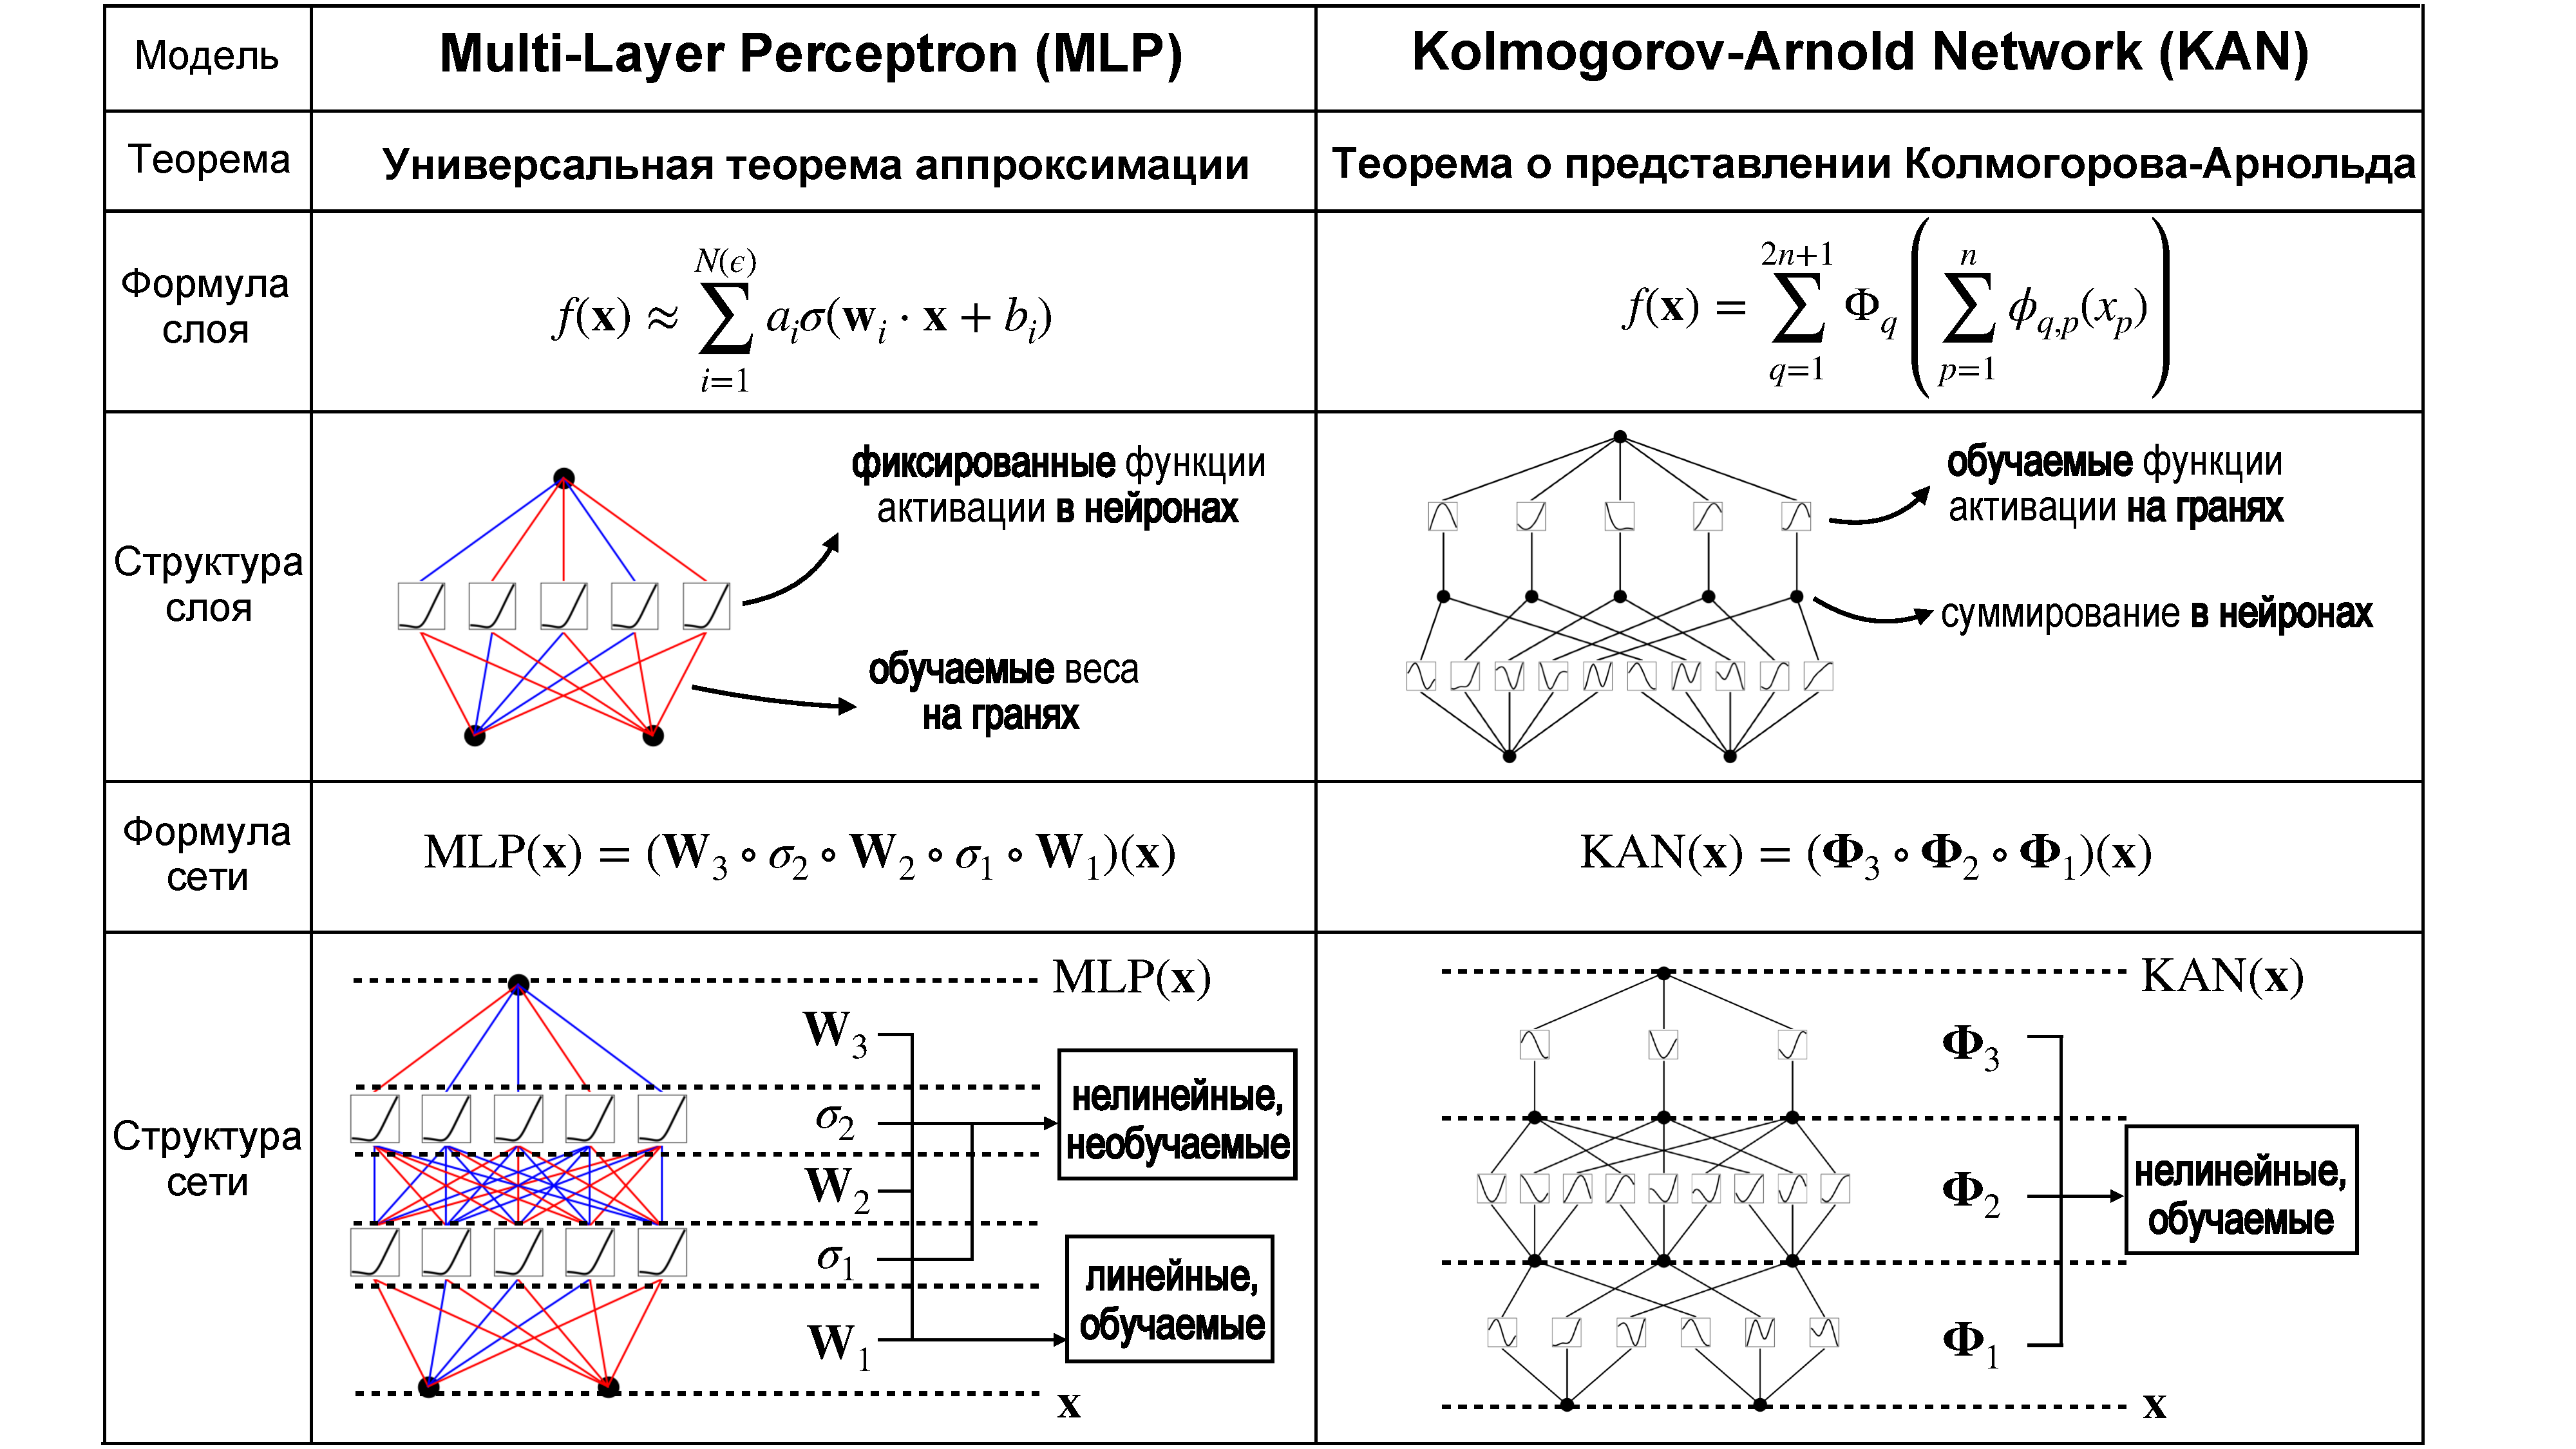
\includegraphics[width=1.1\textwidth]{figures/kan_vs_mlp.pdf}
\end{frame}


% Обязательный слайд: четкая формулировка цели данной работы и постановка задачи
% Описание выносимых на защиту результатов, процесса или особенностей их достижения и т.д.
\begin{frame}{Постановка задачи}
  \textbf{Цель работы}: исследование эффективности применения KAN в сочетании с
  методами противодействия катастрофическому забыванию в условиях непрерывного обучения.
  
  
  \textbf{Задачи}:
\begin{enumerate}
    \item Изучить методы противодействия катастрофическому забыванию и выделить основные подходы, лежащие в их основе.
    \item Адаптировать для архитектуры KAN методы, представляющие каждый из этих подходов.
    \item Применить полученные модели в задаче распознавания образов в условиях непрерывного обучения с использованием набора данных CUB200.
    \item Выяснить путем сравнения моделей, помогают ли особенности KAN повысить эффективность классических приёмов.
    \item Проанализировать полученные результаты и оценить перспективы
        применения KAN в задачах непрерывного обучения.
\end{enumerate}
\end{frame}
            

\begin{frame}{Три основных подхода к противодействию забыванию}
  \begin{center}
    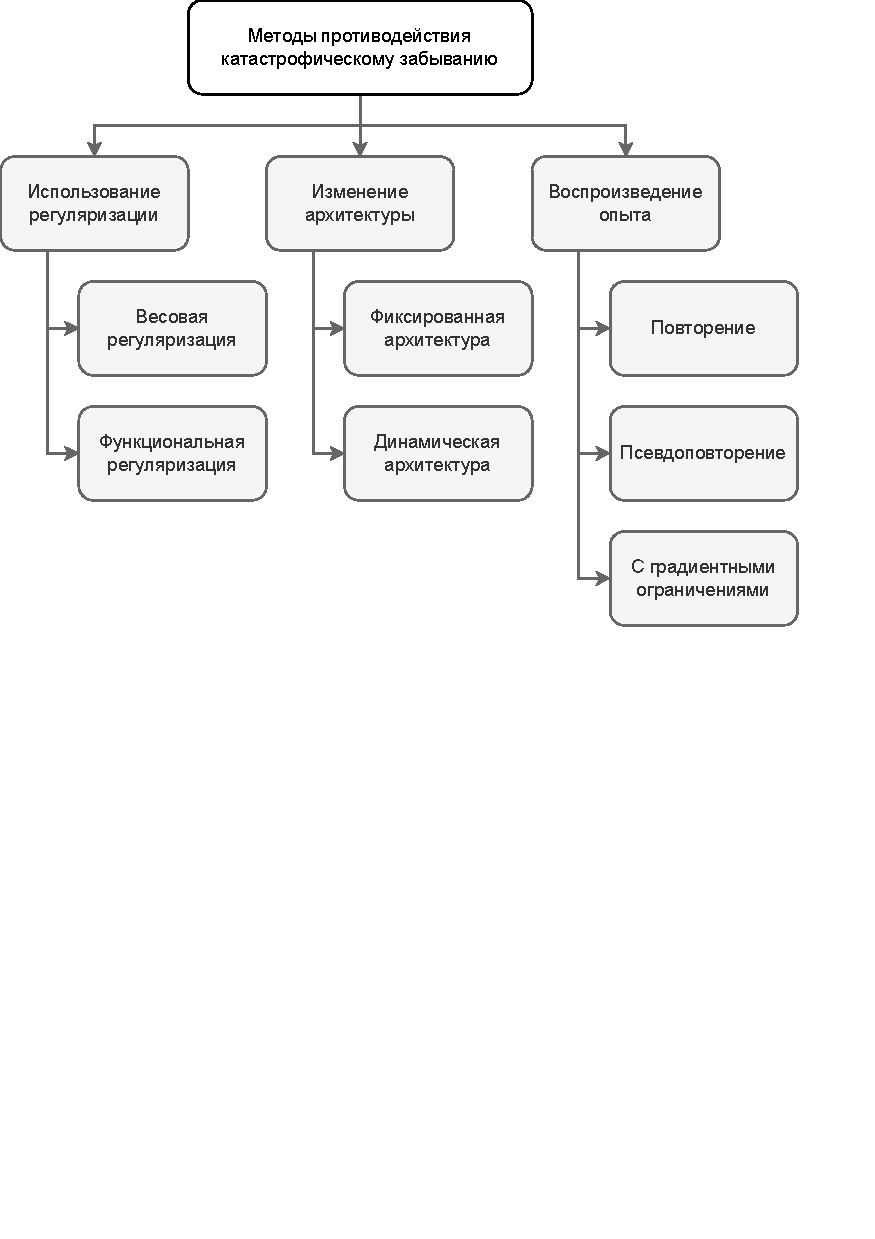
\includegraphics[width=0.8\textwidth]{figures/taxonomy.pdf}
  \end{center}
\end{frame}


\begin{frame}{Отличительные особенности реализованных моделей}
  \begin{enumerate}
    \item \textbf{Оригинальная архитектура} - KAN:
      \begin{itemize}
        \item B-сплайны фиксированного порядка;
        \item Упрощённые функции активации;
        \item Фиксированная сетка базисных функций;
        \item Инициализации параметров с помощью МНК.
      \end{itemize}
    \item \textbf{Подход с использованием регуляризации} - EWC:
      \begin{itemize}
        \item Онлайн обновление;
        \item Адаптивная оценка меток.
      \end{itemize}
    \item \textbf{Подход с изменением архитектуры} - FEL:
      \begin{itemize}
        \item Инициализация весов c помощью He initialization;
        \item Нормализация значений в слое;
        \item Вычисление значений по батчам.
      \end{itemize}
    \item \textbf{Подход с воспроизведением опыта} - GeppNet:
      \begin{itemize}
        \item Инициализация прототипов на базовом наборе данных;
        \item Раздельное обучение SOM и KAN.
      \end{itemize}
  \end{enumerate}
\end{frame}


\begin{frame}{Применение моделей в задачах непрерывного обучения}
  \textbf{Описание используемого набора данных}:
  \begin{table}[h!]
      \begin{center}
          \begin{tabular}{ |c|c|  }
              \hline
              \multicolumn{2}{|c|}{CUB-200-2011} \\
              \hline
              Объект выборки & RGB изображение \\
              \hline
              Количество классов & 200 \\
              \hline
              Количество признаков & 2,048 \\
              \hline
              Размер обучающей выборки & 5,994 \\
              \hline
              Размер тестовой выборки & 5,794 \\
              \hline
              Тренировочные объекты/класс & 29-30 \\
              \hline
              Тестовые объекты/класс & 11-30 \\
              \hline
          \end{tabular}
      \end{center}
  \end{table}
  \textbf{Проведённые эксперименты}:
  \begin{enumerate}
    \item Обучение с перестановкой признаков;
    \item Инкрементальное обучение классам.
  \end{enumerate}
\end{frame}

\begin{frame}{Использованные метрики}
  \vspace{-15pt}
  \begin{equation*}
    \Omega_{base}=\frac{1}{T-1}\sum_{i=2}^{T}\frac{\alpha_{base,i}}{\alpha_{ideal}},
  \end{equation*}
  \begin{equation*}
    \Omega_{new}=\frac{1}{T-1}\sum_{i=2}^{T}\frac{\alpha_{new,i}}{\alpha_{ideal}},
  \end{equation*}
  \begin{equation*}
    \Omega_{all}=\frac{1}{T-1}\sum_{i=2}^{T}\frac{\alpha_{all,i}}{\alpha_{ideal}},
  \end{equation*}
  где:\\
  \(\alpha_{ideal}\) - значение метрики accuracy на всех выборках, полученное при
  оффлайн обучении,\\
  \(\alpha_{base,i}\) - accuracy на первой тренировочной сессии
  после \(i\)-ой тренировочной сессии,\\
  \(\alpha_{new,i}\) - accuracy на \(i\)-ой тренировочной сессии
  после обучения модели на ней же,\\
  \(\alpha_{all,i}\) - accuracy на всех предыдущих тренировочных сессиях.
\end{frame}


\begin{frame}{Результаты экспериментального исследования}
  \begin{itemize}
    \item MLP демонстрирует наилучшие значения почти всех метрик $\Omega$ во всех экспериментах.
    \item Оригинальная архитектура KAN уступает MLP по всем метрикам на 15--20\%;
    \item RegularizedKAN (адаптация EWC) показал лучший результат по $\Omega_{all}$;
    \item Архитектурные особенности KAN либо усиливают забывание, либо делают обучение нестабильным.
    \item Гипотеза о повышении эффективности методов противодействия катастрофическому забыванию для KAN не подтвердилась.
  \end{itemize}
\end{frame}


\begin{frame}{Результаты}
  \begin{enumerate}
    \item Проведён обзор методов противодействия катастрофическому забыванию.
        Выделены три базовых подхода — регуляризация, изменение архитектуры, воспроизведение опыта.
    \item Внесены изменения в программную реализацию KAN. На базе изменённой архитектуры
        созданы RegularizedKAN, ArchitecturalKAN и RehearsalKAN.
    \item Полученные модели применены в условиях непрерывного обучения в задачах с перестановкой данных и инкрементального обучения классам с использованием набора данных CUB200.
    \item Показано, что эффект от применения классических методов противодействия
      катастрофическому забыванию в KAN не больше, чем от их применения в MLP.
    \item Оценены перспективы дальнейшего применения KAN в непрерывном обучении.
        Опровергнута гипотеза о высокой эффективности KAN при использовании
        совместно с методами противодействия катастрофическому забыванию.
  \end{enumerate}
\end{frame}
\end{document}